\chapter{Conceitos Preliminares}\label{chap2}

Este capítulo apresenta os conceitos relacionados aos tópicos de estudo deste trabalho. Na Seção \ref{sec2:wf}, os \textit{workflows} científicos são apresentados. Em seguida, na Seção \ref{sec2:cc}, as nuvens computacionais são abordadas. Por fim, na Seção \ref{sec2:sp} o problema de escalonamento de \textit{workflows} científicos em ambientes de nuvens \hyphenation{computacionais} é apresentado.
% Melhorar a descrição do capítulo

\section{WfCs}\label{sec2:wf}

As tecnologias de \textit{workflow} foram primeiramente adotadas pela comunidade empresarial, nos chamados \textit{business workflows}. Em 1995 a \textit{Workflow Management Coalition} \cite{hollingsworth95a} definiu essa tecnologia como a automação parcial ou total de um processo, durante o qual documentos, informações ou tarefas são passados de um recurso (humano ou computacional) a outro, para que sejam executadas ações de acordo com um conjunto procedural de regras. Essa definição, embora considere o cenário empresarial, concede a visão dos conceitos originais nos quais os \textit{workflows} científicos foram baseados. O termo \textit{workflow} científico (WfC), foi cunhado para descrever a automatização de experimentos científicos executados em ambientes computacionais utilizando as tecnologias de \textit{workflow} \cite{Barker2008}.

Um WfC é composto por uma série de etapas analíticas, que descrevem o processo de experimentação computacional. Esses sistemas fornecem um ambiente para auxiliar a descoberta científica através da combinação entre gerenciamento de dados, análises, simulação, e visualização \cite{Barker2008, bookDeelman}. Alguns exemplos de WfC são: Cybershake \cite{Deelman2006cybershake}, utilizado pela \textit{Southern California Earthquake Center} para caracterizar o risco de terremoto de uma região; Epigenomics \cite{Juve2013}, usado na automação de várias operações de sequenciamento de genomas; e Ligo \textit{Inpiral Analysis} \cite{Brown2007}, empregado pelo \textit{Laser Interferometer Gravitacional Wave Observatory} (LIGO) para analisar os dados obtidos nas observações de ondas gravitacionais. 

Um \textit{workflow} é definido geralmente como um grafo acíclico dirigido (em inglês \textit{Directed Acyclic Graph}, DAG), no qual os vértices representam as etapas do experimento, também chamadas de atividades, e as arestas descrevem as relações de dependências entre estas. As atividades  de um WfC consistem em várias tarefas executáveis, que consomem partes diferentes dos dados (paralelismo de dados) \cite{Liu2014}. Um WfC pode ter centenas ou  mesmo milhares de tarefas, que além de processarem uma grande quantidade de dados (\textit{data-intensive}), também podem executar durante várias horas, ou mesmo dias  (\textit{compute-intensive}) \cite{Juve2013}.

A Figura \ref{fig:wfexec} representa um \textit{workflow}  composto por três atividades ($A_{i}, A_{k}$ e $A_{y}$). Como pode ser visto, as atividades $A_{i}$ e $A_{y}$  são executadas por $n$ tarefas ($n > 0$), e a atividade $A_{k}$ é executada por uma única tarefa. A relação de precedência entre as tarefas é definido por meio de troca de dados. Portanto, como os dados de saída de uma tarefa são os de entrada de outra, a tarefa só pode ser executada quando todos os seus dados de entradas estiverem disponíveis. Por exemplo, na Figura \ref{fig:wfexec} a tarefa $t_{k_{1}}$ tem relação de dependência com todas as tarefas de $A_{i}$ e, portanto, só poderá ser executada quando todas as tarefas de $A_{i}$ estiverem finalizadas. 

\begin{figure}[!ht]
\centering
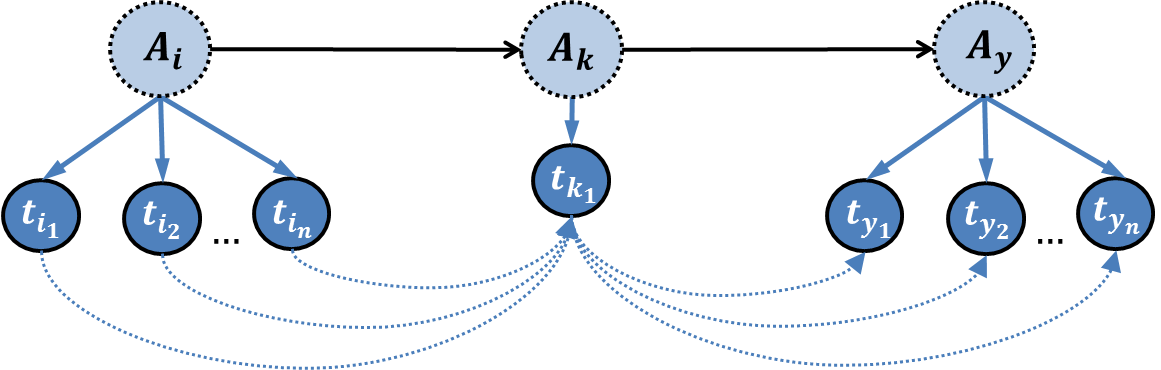
\includegraphics[width=0.8\linewidth]{figure/wf_exec.png}
\caption{Representação das tarefas de um \textit{Workflow} Científico.}
\label{fig:wfexec}
\end{figure}

% FALAR DO Sistema de Gerenciamento de Workflows Científicos.




\section{Nuvens Computacionais}\label{sec2:cc}
Ao longo dos últimos anos várias definições para nuvens computacionais foram apresentadas \cite{Dikaiakos09, Armbrust10, Vaquero08}. Essas definições variam entre o ponto de vista técnico, que aborda os conceitos relacionados a arquitetura e a implementação do ambiente físico e virtual, e o ponto de vista de usabilidade, focado essencialmente nos serviços prestados e nos modelos de cobrança \cite{juve09}. Segundo a ótica de serviço, as nuvens computacionais são um conjunto de servidores virtuais que trabalham interligados através da Internet, e podem ser dinamicamente gerenciados e monitorados \cite{hoffa08}. Esses ambientes se assemelham aos \textit{clusters} nos aspectos técnicos, porém, diferente destes, os recursos computacionais são oferecidos através de virtualização e seguem o modelo de pagamento pague-pelo-uso (do inglês, \textit{pay-per-use}), no qual os usuários são cobrados pelo tempo de uso dos recursos contratados \cite{juve09}.  
 
As nuvens computacionais oferecem várias vantagens técnicas e econômicas em relação as outras plataformas (como \textit{grids} e \textit{clusters}), pois combinam virtualização e escalabilidade em modelos de serviços economicamente viáveis \cite{juve09}. Entre as principais vantagens do uso desse ambiente estão \cite{Hashem15}: processamento paralelo sob demanda; ilusão de recursos infinitos;  e serviços integrados de processamento de dados e armazenamento escalável. Segundo Hashem \textit{et al.} \cite{Hashem15}, além do potencial em diminuir os custos ligados a automação e processamento de dados para indivíduos e empresas, as nuvens computacionais podem reduzir significantemente os custos de aquisição, manutenção, gerenciamento e acesso a infraestruturas computacionais. 

Os serviços prestados pelas nuvens são divididos em três categorias \cite{Hashem15}:

\begin{itemize}
    \item Plataforma como serviço (PaaS, do inglês \textit{Platform as a Service}), que consiste em diferentes recursos (sistemas operacionais, bibliotecas, compiladores, etc.) operando em conjunto para fornecer uma plataforma ao usuário final. Google Apps Engine \cite{gappEngine} e Microsoft Azure \cite{msazure}, são exemplos deste serviço.
    \item \textit{Software} como serviço (SaaS, do inglês \textit{Software as a Service}), consiste em aplicações operadas remotamente em uma infraestrutura de nuvem e oferecidas como um serviço. Exemplos deste modelo são Google Docs \cite{docs}, Gmail \cite{gmail}, Sharelatex \cite{sharelatex}, etc.
    \item Infraestrutura como serviço (IaaS, do inglês \textit{Infrastructure as a Service}, refere-se a equipamentos de \textit{hardware} virtualizados que são fornecidos sob demanda por um provedor de nuvem. Neste modelo, o cliente tem controle total de configuração e instalação de \textit{softwares} no \textit{hardware} adquirido. Amazon EC2 \cite{AmazonEC2}, Google Cloud Platform \cite{gcloud}  e Microsoft Azure \cite{msazure} são exemplos de IaaS.
\end{itemize}


A virtualização é umas das principais tecnologias por trás do sucesso das nuvens computacionais, e pode ser definida como um processo de compartilhamento de recursos computacionais (como CPU, espaço de armazenamento e rede) que isola o \textit{hardware} físico, diminuindo a ineficiência na alocação e distribuição de seus recursos \cite{Hashem15}. O uso mais comum de virtualização é através das máquinas virtuais (MVs), que criam ambientes de \textit{hardware} e \textit{software} configurados de forma totalmente independente do recurso físico, o que permite que várias MVs independentes sejam executadas ao mesmo tempo sob um mesmo \textit{hardware} \cite{hoffa08}. A Amazon EC2, por exemplo, utiliza MVs para oferecer \textit{hardware} virtualizado com diferentes capacidades de memória, largura de banda e poder de processamento. As MVs são classificadas conforme o propósito de uso e capacidade de recursos, e apresentam custo monetário variável. Atualmente, A MV mais barata oferecida pela Amazon EC2 é chamada de t2.nano, e custa $\$0.0059$ hora. A máquina contém um processador virtual (vCPU) baseado no Intel Xeon e 500MB de memória RAM. Já a máquina mais cara, chamada de d2.8xlarge, tem custo de $\$5.52$ hora, 36 vCPUs (também baseadas  no Intel Xeon) e 244 GB de memória RAM \cite{AmazonEC2}.

O uso dos serviços de nuvem para o processamento de aplicações distribuídas se baseia no modelo e IaaS e é feito através da alocação de um \textit{cluster} virtual, que pode ser composto por máquinas de um mesmo tipo (ambiente homogêneo) ou por máquinas com diferentes configurações (ambiente heterogêneo). Especificamente no caso dos WfCs, o SGWfC é responsável pela alocação das MVs necessárias e pelo planejamento de execução das tarefas do \textit{workflow}, feito pelos algoritmos de escalonamento.

                                                                          
\section{O Problema de Escalonamento de WfCs}\label{sec2:sp}

Segundo Yu \textit{et al.} \cite{Yu2008}, escalonamento é o processo de mapear e gerenciar a execução de tarefas em um ambiente computacional. Portanto, é papel do escalonador definir onde e quando  uma tarefa deverá ser executada, sendo que essa decisão está sujeita às restrições impostas às aplicações e ao ambiente. Segundo Topcuoglu \textit{et al.} \cite{HEFT}, em sistemas distribuídos, o escalonamento eficiente das tarefas é um fator chave para atingir um alto desempenho computacional.

Formalmente, o objetivo do escalonador é alocar um conjunto de tarefas $N = \{tf_1,\allowbreak tf_2,\allowbreak\dots,tf_n\}$ em um conjunto de máquinas $M = \{mv_1, mv_2, \dots, mv_n\}$. O escalonador deve otimizar uma função objetivo $f$, que qualifica a solução encontrada e está sujeito a restrições que, caso não sejam satisfeitas, inviabilizam a solução de escalonamento \cite{tsai14}. Os objetivos mais comuns no escalonamento de WfCs são: minimizar o tempo de execução (\textit{makespan}); minimizar o custo monetário; maximizar o uso dos recursos (balanceamento de carga); e minimizar a ocorrência de falhas. No caso das restrições, limitar o orçamento e definir um prazo de execução, são comumente empregadas \cite{Masdari16}. 

O escalonamento de tarefas em sistemas distribuídos faz parte dos chamados problemas NP-Difícil \cite{Ullman1973}. Isso significa que não há algoritmo conhecido capaz de produzir soluções ótimas em tempo polinomial (a menos que $P=NP$). Por conta disso, as abordagens de escalonamento utilizam geralmente algoritmos de resultado aproximados, chamados de  heurísticas de escalonamento \cite{HEFT, Masdari16, Yu2008}. Essas abordagens não garantem que a solução encontrada seja ótima, isto é, a melhor solução possível para o problema. No entanto, são capazes de encontrar soluções com qualidade aceitável, em tempo viável de execução \cite{Kalra15}. As heurísticas são classificadas em diferentes categorias, conforme o critério utilizado na manipulação das tarefas. Uma dessas categorias são os métodos randômicos de busca guiados, chamados também de metaheurísticas \cite{Kalra15, Bossaid13, tsai14}. Segundo Boussaïd \textit{et al.} \cite{Bossaid13}, metaheurísticas são algoritmos elaborados para resolver, de forma aproximada, um grande número de problemas difíceis de otimização sem que seja necessário realizar adaptações profundas no algoritmo para cada um destes problemas. 

Os algoritmos de escalonamento podem ser estáticos ou dinâmicos \cite{Fakhfakh14}. Nos algoritmos estáticos todo o plano de escalonamento é definido antes de qualquer execução. Para isso, os algoritmos consideram as condições iniciais do ambiente (como capacidades de processamento, número de máquinas e taxas de transferência) e não preveem mudanças destas condições ao longo da execução.  Portanto, todas as informações relacionadas ao \textit{workflow} e ao ambiente, como tempo de execução das tarefas, tamanho dos dados e relações de dependências, devem ser conhecidas \textit{a priori} e fazem parte da entrada do problema. A acurácia dessas informações influencia diretamente no resulto do escalonamento, já que informações discrepantes induzem o escalonador ao erro e resultam em soluções de baixa qualidade. As formas mais comuns de obter essas informações é através de execuções prévias do \textit{workflow}, ou com estimativas por modelos matemáticos e testes de \textit{benchmark}.

Nos algoritmos dinâmicos, o escalonamento  é realizado durante a execução do \textit{workflow}. Nessa abordagem, as tarefas são escalonadas por etapas, conforme a disponibilidade do ambiente e das tarefas. Para isso, o escalonador monitora o status de execução e das máquinas e, caso haja tarefas prontas para serem escalonadas e máquinas ociosas, submete as tarefas para a execução conforme um critério de escalonamento que atenda ao objetivo desejado. Normalmente, essa abordagem é local, isto é, o escalonador utiliza as informações das tarefas prontas e das máquinas livres para determinar a alocação, e não considera todo o \textit{workflow} na decisão \cite{Fakhfakh14, Kalra15}. Diferente do escalonamento estático, as informações utilizadas no escalonamento são atualizadas de tempos em tempos, o que melhora a acurácia delas, já que as ocilações de qualidade do ambiente são facilmente detectadas e o escalonamento pode ser adaptado. Embora o escalonamento dinâmico seja mais flexível e exija menos parâmetros de entrada, seu \textit{overhead} de execução e a complexidade na implementação são maiores quando comparados aos algoritmos de escalonamento estático \cite{Fakhfakh14}.




